\documentclass[oneside]{VUMIFPSkursinis}
\usepackage{algorithmicx}
\usepackage{algorithm}
\usepackage{algpseudocode}
\usepackage{amsfonts}
\usepackage{amsmath}
\usepackage{bm}
\usepackage{caption}
\usepackage{color}
\usepackage{float}
\usepackage{graphicx}
\usepackage{listings}
\usepackage{subfig}
\usepackage{wrapfig}

\university{Vilniaus universitetas}
\faculty{Matematikos ir informatikos fakultetas}
\department{Programų sistemų katedra}
\papertype{Laboratorinis darbas I}
\title{Automatinė ūkio valdymo sistema}
\titleineng{Automatic farm management system}
\status{2 kurso 3 grupės studentai}
\author{Matas Savickis}
\secondauthor{Justas Tvarijonas}  
\thirdauthor{Greta Pyrantaitė}   
\fourthauthor{Rytautas Kvasinskas}
\supervisor{Karolis Petrauskas, Doc., Dr.}
\date{Vilnius – \the\year}

% Nustatymai
%\setmainfont{Palemonas}   % Pakeisti teksto šriftą į Palemonas (turi būti įdiegtas sistemoje)
\bibliography{bibliografija}

\begin{document}
\maketitle

\tableofcontents



\sectionnonum{Įvadas}
Pasirinkome programuoti Automatinę ūkio valdymo sistemą(toliau - Auto ūkis) JAVA programavimo kalba, nes visi komandos nariai turėjo pakankamas žinias programuoti šia kalba ir kalbos funkcionalumas, mūsų manymu, atitiko poreikius. Programuodami pirmą sistemos variantą stengėmės prisilaikyti bendrų objektinio programavimo principų ir JAVA kodo standarto. Apie patį sistemos projektavimą pagalvojome minimaliai dėl tuo metu neturimų žinių. UML diagramų braižymui naudojome www.planttext.com(toliau - PlantText) ir www.draw.io.

\sectionnonum{Žodynas}
\begin{itemize}
	\item Klasės:
		\begin{itemize}
			\item[*] AutoŪkis - pagrindinė(main) programos klasė. Ši klasė piešia grafinę vartotojo sąsaja ir laiko savyje kitų klasių objektus kurių informacija reikalinga piešimui
			\item[*] Map - teritorijos piešimui skirta klasė.
			\item[*] ŽemėsTeritorija - apskaičiuoja tam tikros teritorijos plotą.
 			\item[*] Gyvūnas - klasė skirta gyvūno rodmenims ir metodams saugoti
			\item[*] AriamasLaukas - laiko savyje reikšmes apibūdinančias unikalų lauką ir metodus susijusius su lauko darbu.
			\item[*] Ganykla - laiko parametrus ir metodus darbui su ganyklomis kurios yra žemės plote.
			\item[*] ŪkinisPastatas - saugo ūkinius 
			\item[*] ŪkioTechnika - laiko ūkio technikos charakteristikos reikšmes. Apskaičiuoja technikos judėjimo greitį.
			\item[*]Žemės parametrai - saugo įvairius žemės parametrus(drėgmė, ph...).
			\item[*] Orai - klasė skirta pasiimti orų prognozes iš www.gismeteo.lt kurių paprašo vartotojas.
			\item[*] Žemės detektorius - klasė skirta bendrauti su žemės detektoriumi

		\end{itemize}
	\item Bendri terminai:
		\begin{itemize}
			\item Žemės plotas - vieta kurią valdo ir gali stebėti vartotojas(ūkininkas) 
		\end{itemize}
\end{itemize}

\section{Sukurtos sistemos aprašymas(v1.0)}

\subsection{Loginis pjūvis}
	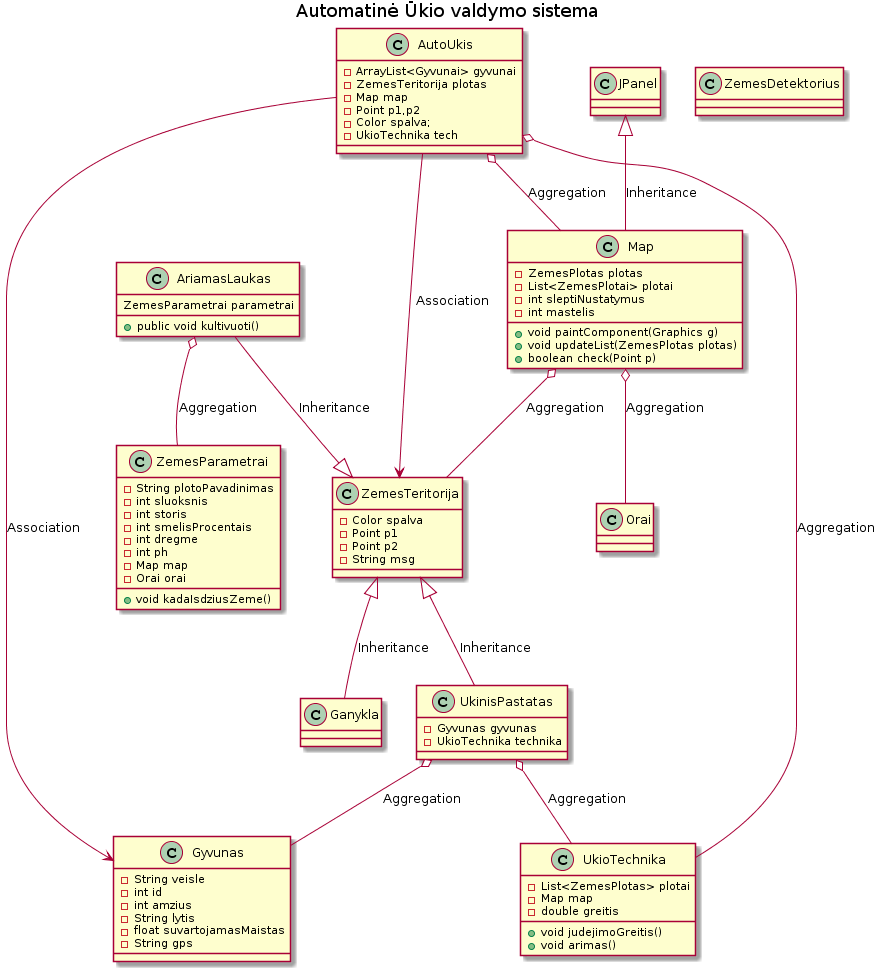
\includegraphics[width=\textwidth,height=\textheight,keepaspectratio]{uml.png}	
	Pagal suprogramuotą šabloninį programos karkasą nubraižėme UML diagramą minėta PlnatText programa.
	\begin{itemize}
		\item Dizainas: 
		\begin{itemize}
			\item Pagrindinė klasė yra AutoUkis.form. Joje sukurtas ir aprašytas Graphical User Interface (GUI), visas vartotojo bendravimas su programa vyksta per ją, nes per ją pasiekiami visi duomenys iš kitų klasių, pavyzdžiui duomenys, esantys klasėje Gyvūnas, kurioje įrašoma vartotojo įvesta informacija apie gyvūną (veislė, amžius, t.t.). Taip pat AutoUkis klasėje kuriama dauguma objektų ir jie ten laikomi, sudedami į sąrašus. Visos kitos klasės turi savo atskiras paskirtis, tokias kaip žemėlapio braižymas, oro prognozių sekimas ir įvairių parametrų laikymas. Kai kurios klasės (pvz. ZemesDetektorius) buvo sukurtos vėlesniam panaudojimui, bet šiuo metu nėra niekur panaudotos.
Dėl to, ką būtų buvę galima daryti kitaip, GUI perkėlimas į atskirą klasę padarytų programą skaitomesnę ir tvarkingesnę, būtų lengviau rasti atskirą kodą. Dar viena alternatyva būtų įgyvendinti front-end dalį web aplinkoje, bet šiuo metu nematome tam būtinybės.
		\end{itemize}
		\item Funkcionalumas:
		\begin{itemize}
		\item Viso užsibrėžto programos funkcionalumo įgyvendinti nepavyko. Kai kurios klasės buvo sukurtos ateityje planuojamoms funkcijoms, kurios dar nėra implementuotos. Programa kol kas veikia tik ant kompiuterio ir vienintelis jos bendravimas su internetu yra per Orai klasę, kuri skirta vartotojo pasirinkto miesto orų prognozėms gauti iš gismeteo.lt svetainės. Klasėse Gyvunas, Map, ZemesTeritorija ir iš jos išeinančiose klasėse saugomi atitinkami duomenys apie sukurtus objektus bei aprašyti dar neišplėtoti metodai, tokie kaip žemės teritorijos žymėjimas. Planuojama, kad klasė ZemesDetektorius generuos atsitiktinius parametrus, kurie bus perduoti ZemesParametrai klasei.
Nepilnai įgyvendintas finkcionalumas ir neišbaigtos klasės sukelia nepatogumų aprašant programą, nes sunku braižyti diagramas, suvokti aiškius ryšius tarp komponentų ir vykdomas funkcijas.
		\end{itemize}	
	\end{itemize}
\subsection{Kūrimo pjūvis}
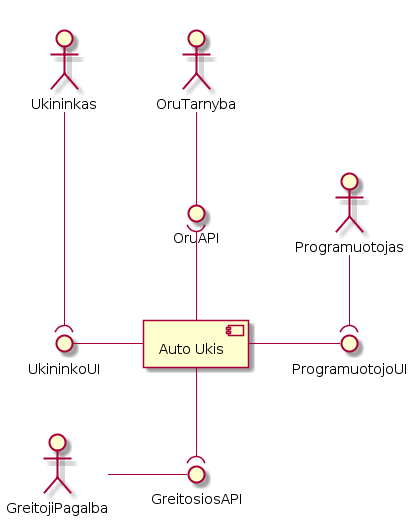
\includegraphics{l0.png}	
	\pagebreak
	\begin{itemize}
		\item Dizainas: 
		\begin{itemize}
			\item Pradėjus rašyti programą nepagalvojome apie kūrimo pjūvį ir kaip teisingiau būtų pradėti viską. Žiūrint dabar visa programa buvo pradėta kurti pagal Bottom -> Up principą. Iš pradžių apsirašėme daugybę mažų klasių ir paskui jas bandėme apjungti į didesnę sistemą. Išskyrėme tokius komponentus kaip ūkininkas, programa, orų tarnyba, žemės detektorius ir administratorius. Kiekvienas komponentas turi skirtingas prieigas prie informacijos ir skirtingas funkcijas, reikalingas ūkio visapusiškam funkcionavimui. Kai kurios klasės liko nepanaudotos, nes šiuo metu jos neatrodo pakankamai svarbios pradiniam projekto variantui. Ūkiniko, Admin ir darbuotojo panelės įtrauktos į dokumentaciją norint pavaizduoti skirtingas prieigas prie sistemos.
		\end{itemize}
		\item L0:
		\begin{itemize}
			\item Šioje diagramoje pavaizdavome sistemos bendravimą su išoriniais agentais tokiais kaip Greitoji pagalba, Ūkininkas ir t.t. . Ši diagrama aiškiai ir paprastai parodo kuriamus ir įgyvendinamus interfeisus. Galbūt būtų galima Greitosios Pagalbos interfeisą išskaidyti į kelis detalesnius interfeisus, bet apskritai didelių problemų nepastebime.

		\end{itemize}
	\end{itemize}
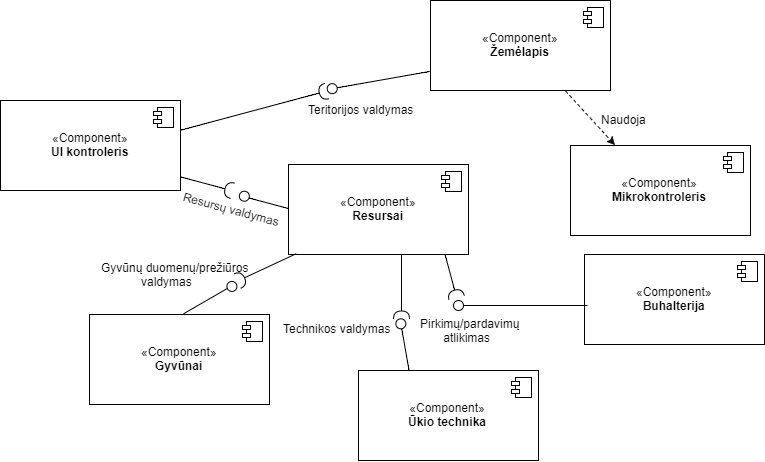
\includegraphics[width=\textwidth,height=\textheight,keepaspectratio]{l1.png}	

\begin{itemize}
	\item L1: Sudėjus komandos idėjas apie tai, kaip turėtų atrodyti L1 diagrama, supratome, kad mūsų sistema neturi normalios struktūros ir gerai nebuvome pagalvoję kaip visi komponentai siesis vieni su kitais, todėl ir diagrama atrodo chaotiška. Trūksta konkretumo kaip turi Admin sietis su kitas komponentais. Programa atsiranda kaip komponentas  kas greičiausiai yra nekorektiška.

\end{itemize}
	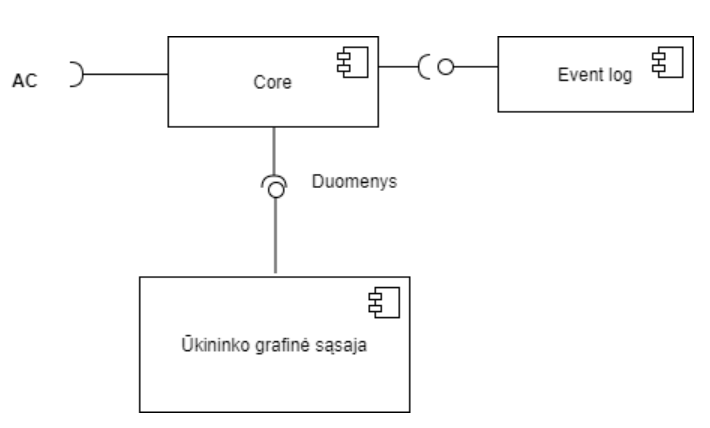
\includegraphics[width=\textwidth,height=\textheight,keepaspectratio]{l2uki.png}

	\begin{itemize}
		\item L2(Ūkininkas): Šioje diagramoje parodyta, kad programos pagrindas kuria suteikia interface’a grafinei vartotojo sąsajai. Paduoti duomenys yra užregistruojami Event Log’e.

	\end{itemize}
	
	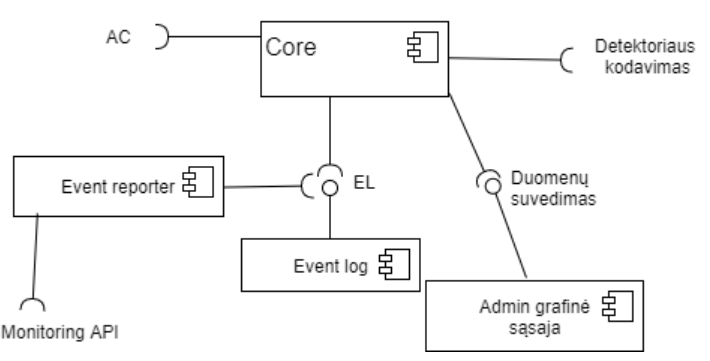
\includegraphics[width=\textwidth,height=\textheight,keepaspectratio]{l2admin.png}
	
	\begin{itemize}
		\item L2(Admin): Šioje diagramoje parodyta,kad programos pagrindas naudoja duomenų suvedimo interface, kurį suteikia admin grafinė sąsaja, bei naudoja Detektoriaus kodavimo interface. Visus įvykius įrašo į event log

	\end{itemize}

		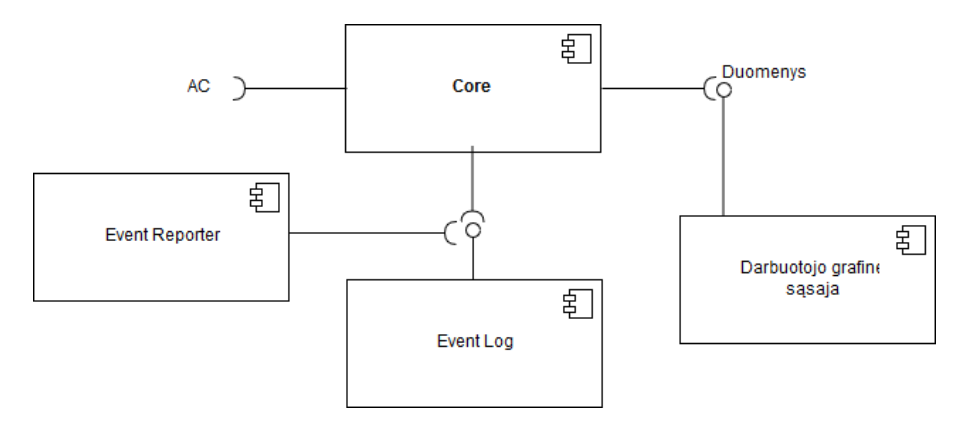
\includegraphics[width=\textwidth,height=\textheight,keepaspectratio]{l2darb.png}

\begin{itemize}
		\item L2(Darbuotojas):Šioje diagramoje parodyta, kad programos pagrindas  grafinę sąsają ir perduoda duomenis į event log’ą. 

	\end{itemize}

		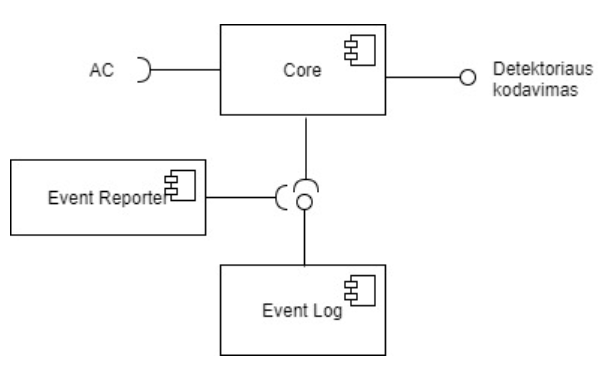
\includegraphics[width=\textwidth,height=\textheight,keepaspectratio]{l2det.png}

\begin{itemize}
		\item L2(Detektorius): ši diagrama vaizduoja detektoriaus išvedamus duomenis. Įvykiai įrašomi Event Log’e.
	\end{itemize}
\pagebreak
		

	
\subsection{Use case}
\subsection{Proceso pjūvis}
\subsection{Fizinis pjūvis}
	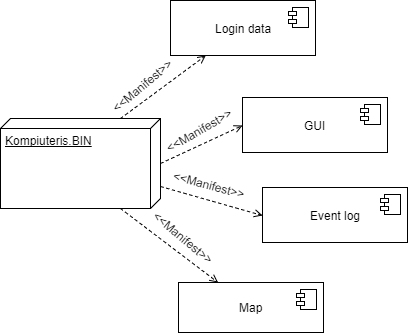
\includegraphics[width=15cm,height=10cm]{Deployment.png}
	\begin{itemize}
		\item D0: Šioje diagramojo parodyta, kas saugoma device kompiuteris. 
		Iš diagramos matome, kad šiame įrenginyje saugomi prisijungimo duomenys, Vartotojų grafinės sąsajos, teritorijos žemėlapis bei programojo atliktų veiksmų išrašas. Alternatyva buvo saugoti šiuos duomenis išnuomuotame web service, tačiau daug negalvoję nusprendėme duomenis saugoti kompiuteryje.
	\end{itemize}
	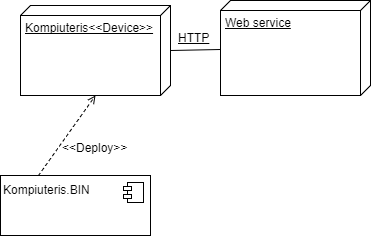
\includegraphics[width=15cm,height=10cm]{Deployment0.png}
	\begin{itemize}
		\item D1: Tai bendresnė D0 diagrama, joje matome, kad kompiuteris bendrauja su web HTTP ryšiu norėdamas gauti pranešimus apie orus.
	\end{itemize}

\section{Perprojektuotos sistemos aprašymas(To-Be, v2.0)}

\subsection{Loginis pjūvis}
\subsection{Kūrimo pjūvis}
\subsection{Use case}
\subsection{Proceso pjūvis}
\subsection{Fizinis pjūvis}



\sectionnonum{Rezultatai ir išvados}



\end{document}
